\section{GenSim}

\subsection{The GenSim ADL}

\begin{frame}{The GenSim ADL}

\end{frame}

\begin{frame}{The GenSim ADL}

GenSim is the name of our ADL toolset. It is designed to:

\begin{itemize}
	\item ... be intuitive and easy to learn
	\item ... create high performance simulation tools\footnote{DAC'13: \url{https://doi.org/10.1145/2463209.2488760}}
	\item ... be extensible in terms of analyses

\end{itemize}

\end{frame}

\begin{frame}{GenSim Toolflow}

\centering
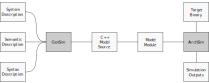
\includegraphics[width=\textwidth]{figures/gensim-toolflow}

\end{frame}

\begin{frame}{GenSim Model Components}

A GenSim description consists of three components
\pause

\begin{minipage}[h]{0.6\textwidth}
\begin{itemize}
\item A `System' component
\begin{itemize}
\item Available instruction sets
\item Register file layout
\item Configurable Features
\end{itemize}
\end{itemize}
\end{minipage}%
\begin{minipage}[h]{0.35\textwidth}
\centering
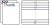
\includegraphics[width=\textwidth]{figures/component-system}
\end{minipage}

\smallskip
\pause

\begin{minipage}[h]{0.6\textwidth}
\begin{itemize}
\item A `Syntax' component
\begin{itemize}
\item Instruction formats
\item Instruction encoding
\end{itemize}
\end{itemize}
\end{minipage}%
\begin{minipage}[h]{0.35\textwidth}
\centering
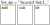
\includegraphics[width=\textwidth]{figures/component-syntax}
\end{minipage}

\smallskip
\pause

\begin{minipage}[h]{0.6\textwidth}
\begin{itemize}
\item A `Semantics' component
\begin{itemize}
\item Instruction behaviours
\item Exception behaviour
\end{itemize}
\end{itemize}
\end{minipage}%
\begin{minipage}[h]{0.35\textwidth}
\centering

\includegraphics[width=\textwidth]{figures/component-semantics}
\end{minipage}

\end{frame}

\begin{frame}{Available Models}

\centering
\begin{columns}
\begin{column}{0.6\textwidth}
\begin{itemize}
	\item ARMv7-A 
	\only<2>{
		\begin{itemize}
			\item ARM + Thumb-2
			\item Some VFP and NEON
			\item User Mode + Full System
		\end{itemize}
	}
	\item ARMv8
	\only<3>{
		\begin{itemize}
			\item AArch64 Only
			\item Some FP Support
			\item User Mode + Full System
		\end{itemize}
	}
	\item RISC-V
	\only<4>{
		\begin{itemize}
			\item Core and FP
			\item User Mode only
		\end{itemize}
	}
	\item x86-64
	\only<5>{
		\begin{itemize}
			\item External decoder
			\item User Mode only
		\end{itemize}
	}
\end{itemize}
\end{column}
\begin{column}{0.4\textwidth}

\only<2>{
\centering
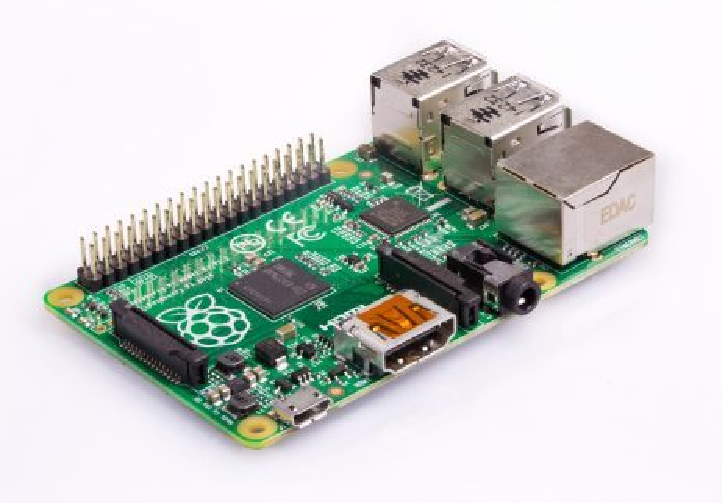
\includegraphics[width=\textwidth]{figures/rpi1}\\
\centering
\tiny{Raspberry Pi Model B}
}
\only<3>{
\centering
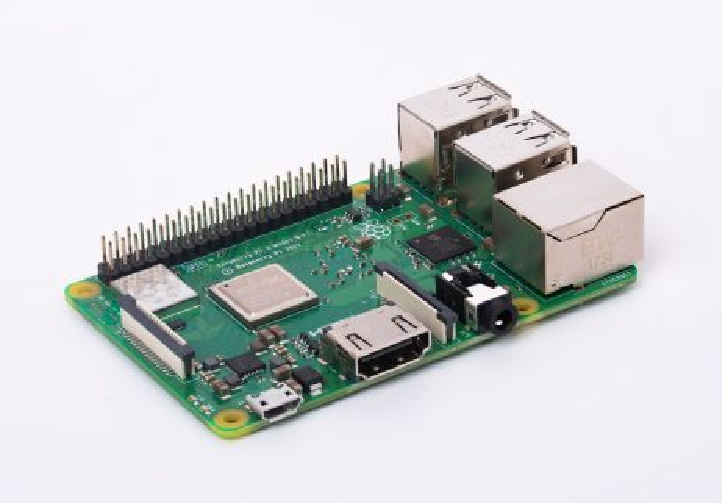
\includegraphics[width=\textwidth]{figures/rpi2}\\
\tiny{Raspberry Pi 3 Model B+}
}
\only<4>{
\centering
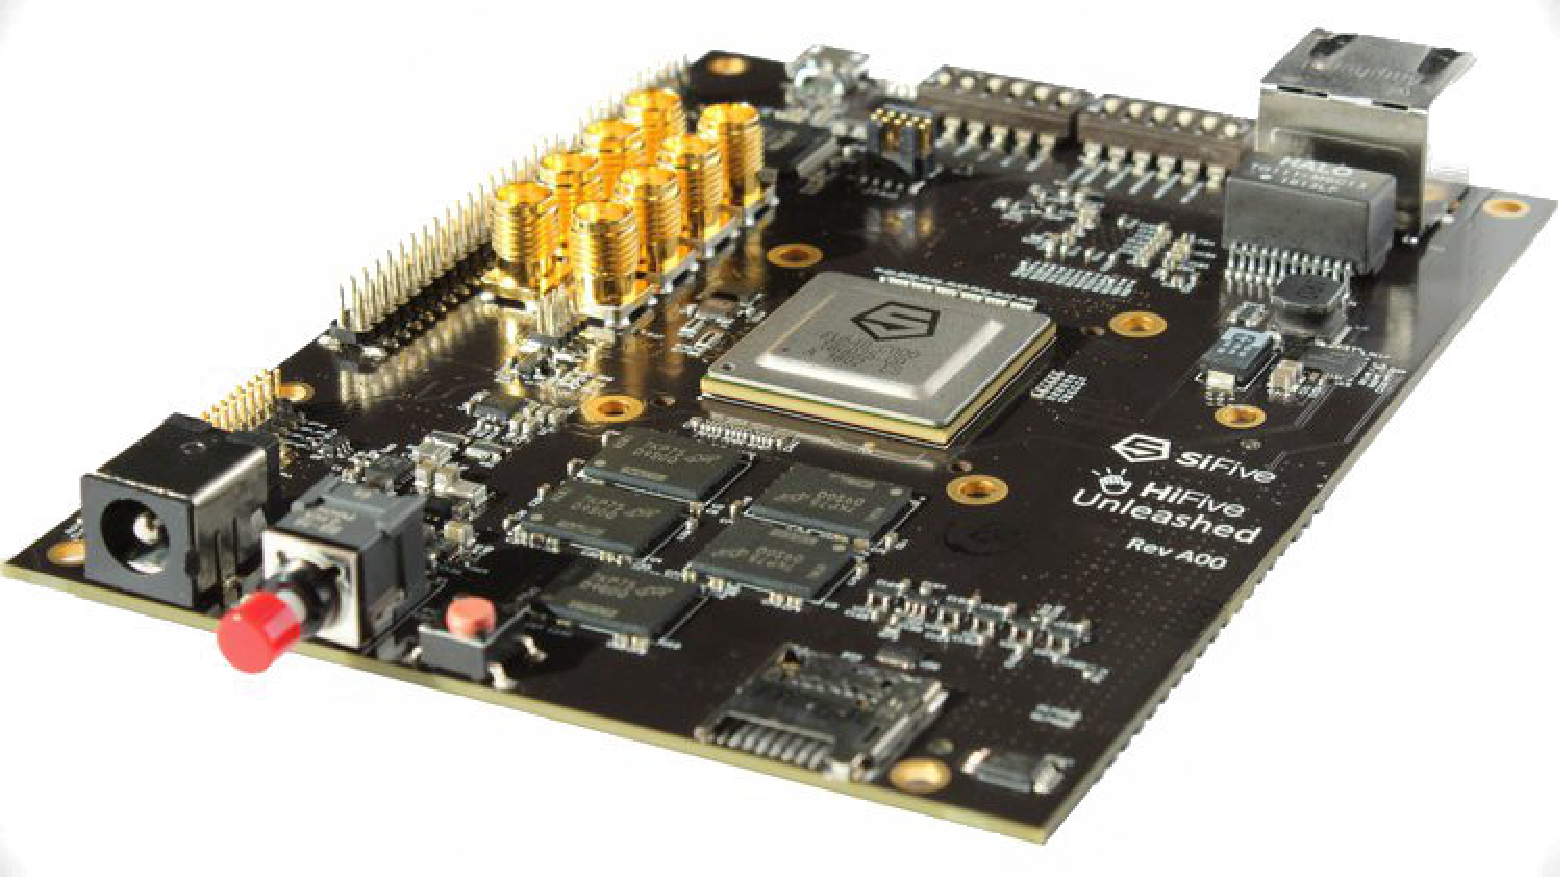
\includegraphics[width=\textwidth]{figures/riscv-sifive}\\
\tiny{SiFive RISC-V SBC}
}
\only<5>{
\centering
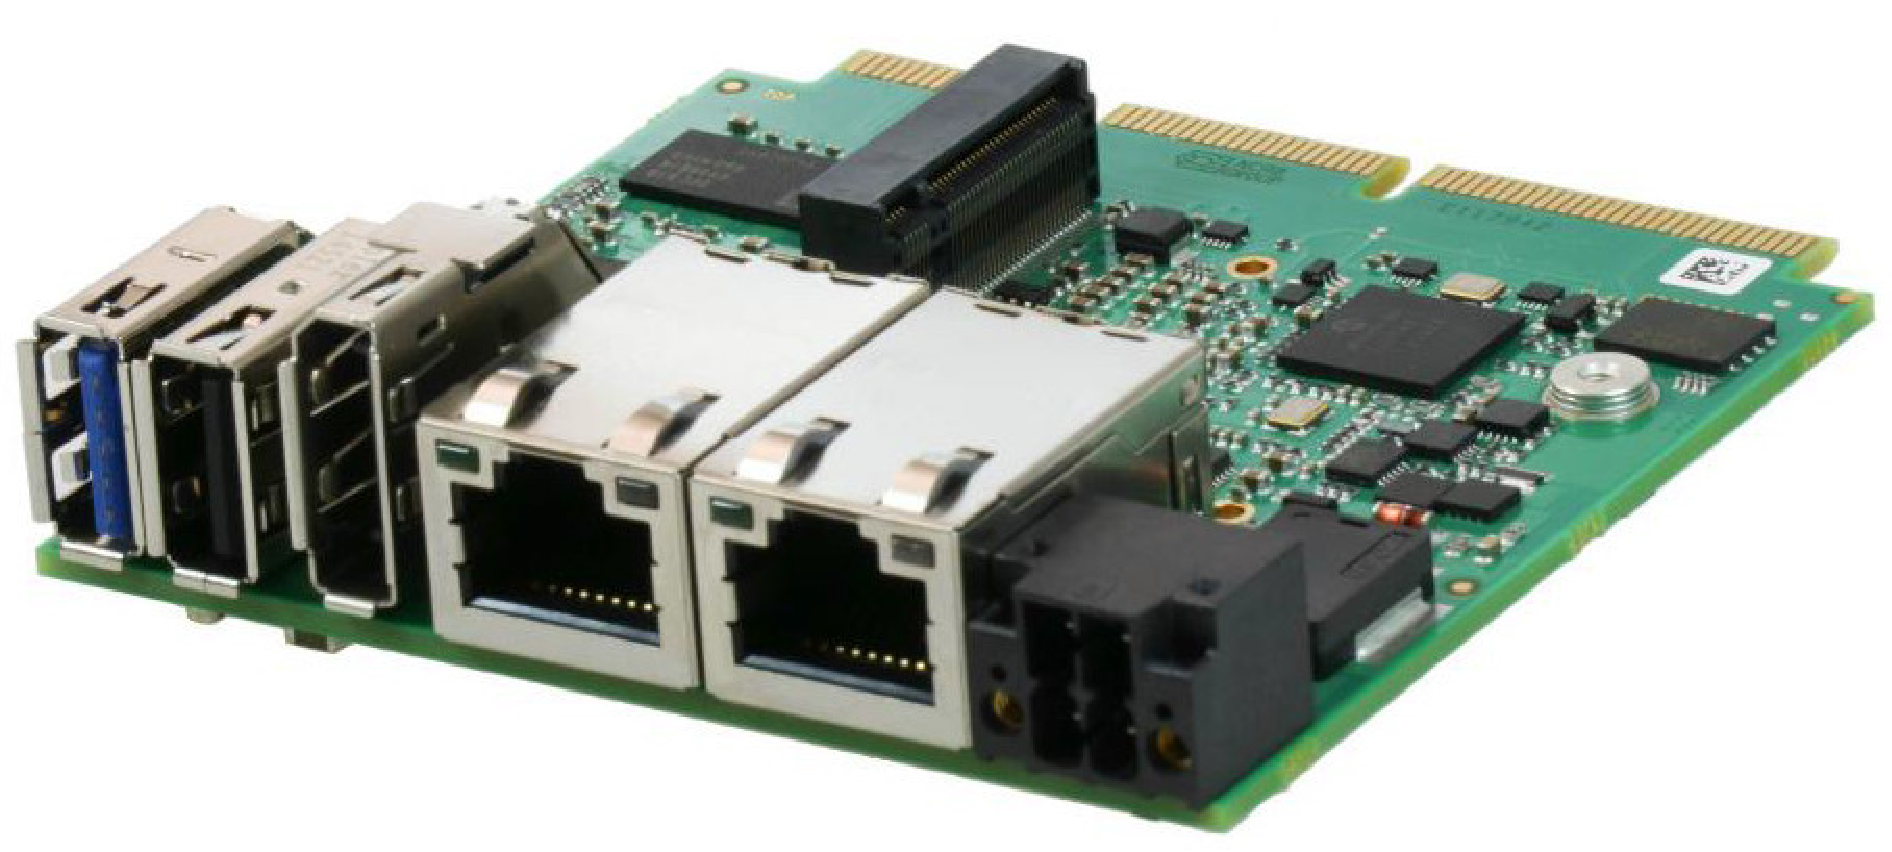
\includegraphics[width=\textwidth]{figures/x86-sbc}\\
\tiny{ADL ADLE3800SEC}
}

\end{column}
\end{columns}

\end{frame}

\begin{frame}{Execution Model}

\begin{minipage}[t][0.4\textheight]{\textwidth}
GenSim generally has a simplistic execution model
\begin{itemize}
	\item Instructions have a straightforward encoding
	\item Instructions are executed in PC order
	\item Effects occur immediately
	\item Instructions can be predicated
\end{itemize}
\end{minipage}

\pause

\begin{minipage}[t][0.4\textheight]{\textwidth}
Which architectures do not fit this model?
\begin{itemize}
	\item x86 (stateful encoding)
	\item MIPS (delay slots)
	\item DSP-like architectures (delayed effects)
\end{itemize}
\end{minipage}

\end{frame}
